\documentclass[letterpaper,9pt,twocolumn,twoside,]{pinp}

%% Some pieces required from the pandoc template
\providecommand{\tightlist}{%
  \setlength{\itemsep}{0pt}\setlength{\parskip}{0pt}}

% Use the lineno option to display guide line numbers if required.
% Note that the use of elements such as single-column equations
% may affect the guide line number alignment.

\usepackage[T1]{fontenc}
\usepackage[utf8]{inputenc}

% pinp change: the geometry package layout settings need to be set here, not in pinp.cls
\geometry{layoutsize={0.95588\paperwidth,0.98864\paperheight},%
  layouthoffset=0.02206\paperwidth, layoutvoffset=0.00568\paperheight}

\definecolor{pinpblue}{HTML}{185FAF}  % imagecolorpicker on blue for new R logo
\definecolor{pnasbluetext}{RGB}{101,0,0} %



\title{Analisis de variables climáticas parámo la Rusia}

\author[a]{Camilo Andres Cruz Sanchez}
\author[a]{Juan David Leon Torres}
\author[a]{Juan Jose Olarte Zapata}
\author[b]{Natali Andrea Lopez Toro}
\author[a]{Cristian Camilo Gañan Tapasco}

  \affil[a]{Departamento de ciencias forestales, Universidad Nacional de Colombia,
Medellín}
  \affil[b]{Área curricular de Medio Ambiente , Universidad Nacional de Colombia,
Medellín}

\setcounter{secnumdepth}{0}

% Please give the surname of the lead author for the running footer
\leadauthor{Cruz; Leon; Olarte; Lopez; Gañan}

% Keywords are not mandatory, but authors are strongly encouraged to provide them. If provided, please include two to five keywords, separated by the pipe symbol, e.g:
 \keywords{  one |  two |  optional |  keywords |  here  }  

\begin{abstract}
Your abstract will be typeset here, and used by default a visually
distinctive font. An abstract should explain to the general reader the
major contributions of the article.
\end{abstract}

\dates{This version was compiled on \today} 

% initially we use doi so keep for backwards compatibility
% new name is doi_footer
\doifooter{Hidrología Forestal}

\pinpfootercontents{Parámo La Rusia}

\begin{document}

% Optional adjustment to line up main text (after abstract) of first page with line numbers, when using both lineno and twocolumn options.
% You should only change this length when you've finalised the article contents.
\verticaladjustment{-2pt}

\maketitle
\thispagestyle{firststyle}
\ifthenelse{\boolean{shortarticle}}{\ifthenelse{\boolean{singlecolumn}}{\abscontentformatted}{\abscontent}}{}

% If your first paragraph (i.e. with the \dropcap) contains a list environment (quote, quotation, theorem, definition, enumerate, itemize...), the line after the list may have some extra indentation. If this is the case, add \parshape=0 to the end of the list environment.


\hypertarget{introducciuxf3n}{%
\section{Introducción}\label{introducciuxf3n}}

\begin{figure}

{\centering 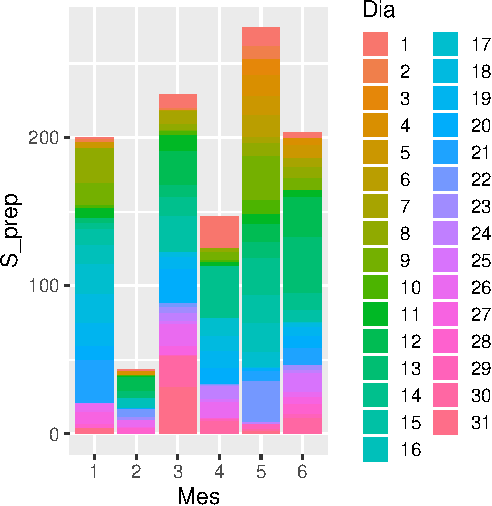
\includegraphics{report_hidrolgy_files/figure-latex/unnamed-chunk-1-1} 

}

\caption{Tendencia Diaría de precipitación}\label{fig:unnamed-chunk-1}
\end{figure}

\begin{figure}

{\centering 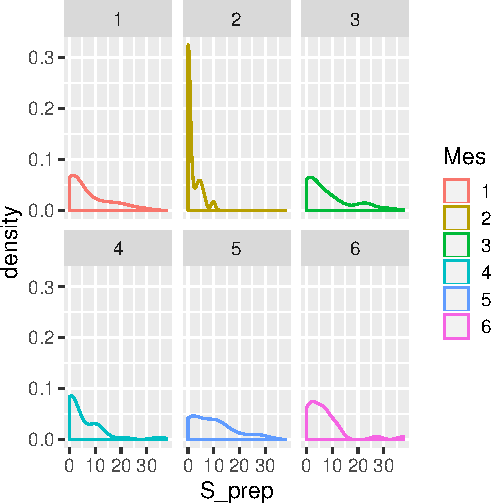
\includegraphics{report_hidrolgy_files/figure-latex/unnamed-chunk-2-1} 

}

\caption{Tendencia Diaría de precipitación}\label{fig:unnamed-chunk-2}
\end{figure}

\begin{figure}

{\centering 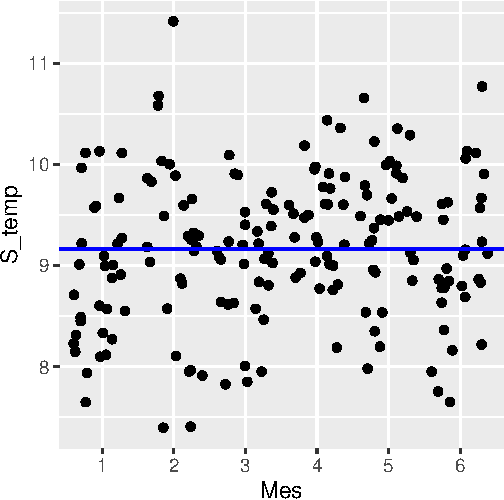
\includegraphics{report_hidrolgy_files/figure-latex/unnamed-chunk-3-1} 

}

\caption{Tendencia de la temperatura mensual}\label{fig:unnamed-chunk-31}
\end{figure}
\begin{figure}

{\centering 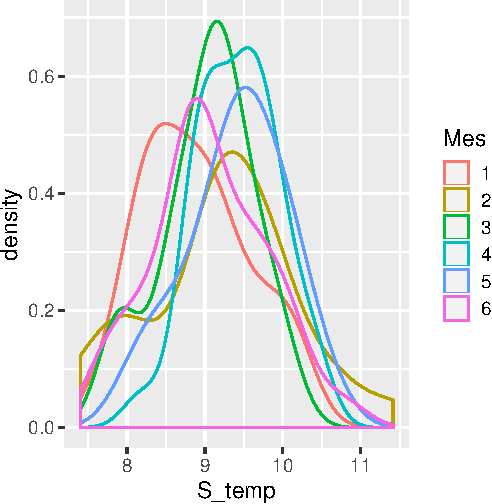
\includegraphics{report_hidrolgy_files/figure-latex/unnamed-chunk-3-2} 

}

\caption{Tendencia de la temperatura mensual}\label{fig:unnamed-chunk-32}
\end{figure}

\begin{figure}

{\centering 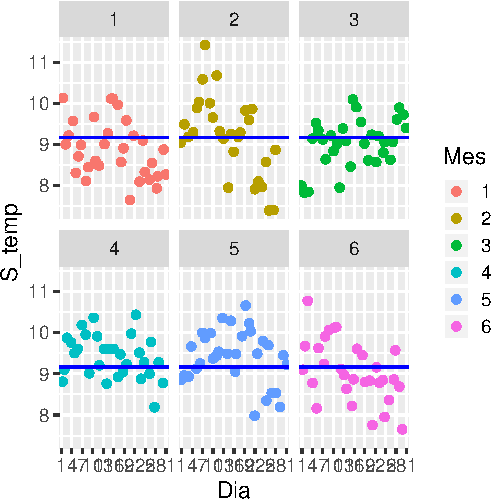
\includegraphics{report_hidrolgy_files/figure-latex/unnamed-chunk-4-1} 

}

\caption{Temperatura media general}\label{fig:unnamed-chunk-4}
\end{figure}

\begin{center}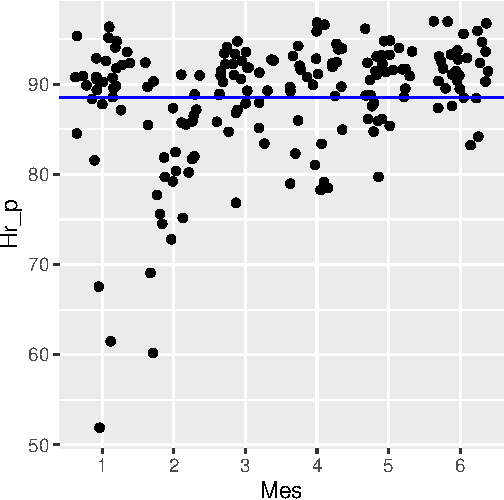
\includegraphics{report_hidrolgy_files/figure-latex/unnamed-chunk-5-1} \end{center}

\begin{center}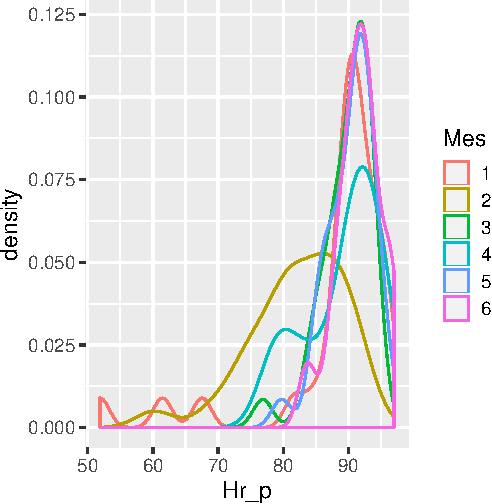
\includegraphics{report_hidrolgy_files/figure-latex/unnamed-chunk-6-1} \end{center}

\begin{center}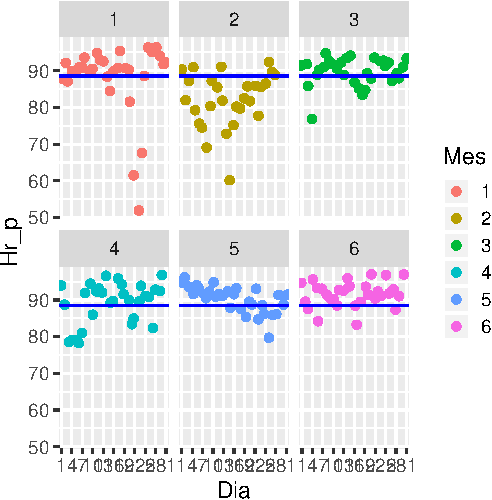
\includegraphics{report_hidrolgy_files/figure-latex/unnamed-chunk-7-1} \end{center}

\begin{center}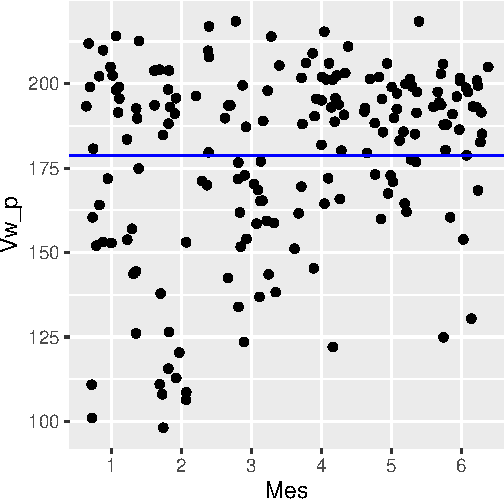
\includegraphics{report_hidrolgy_files/figure-latex/unnamed-chunk-8-1} \end{center}

\begin{center}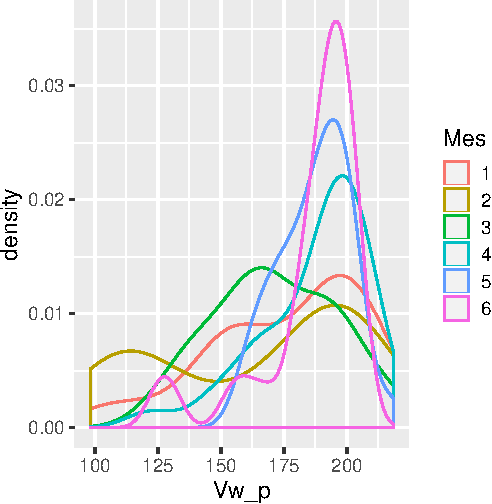
\includegraphics{report_hidrolgy_files/figure-latex/unnamed-chunk-9-1} \end{center}

\hypertarget{materiales-y-muxe9todos}{%
\section{Materiales y métodos}\label{materiales-y-muxe9todos}}

\hypertarget{localizaciuxf3n-y-descripciuxf3n-del-uxe1rea-de-estudio}{%
\subsection{Localización y descripción del área de
estudio}\label{localizaciuxf3n-y-descripciuxf3n-del-uxe1rea-de-estudio}}

\hypertarget{levantamiento-de-informaciuxf3n}{%
\subsubsection{1) Levantamiento de
información}\label{levantamiento-de-informaciuxf3n}}

\hypertarget{procesamiento-de-los-datos-recolectados}{%
\subsubsection{2) Procesamiento de los datos
recolectados}\label{procesamiento-de-los-datos-recolectados}}

\hypertarget{resultados-y-discusiuxf3n}{%
\section{Resultados y Discusión}\label{resultados-y-discusiuxf3n}}

%\showmatmethods


\renewcommand\refname{Conclusiones}
\bibliography{pinp}
\bibliographystyle{jss}



\end{document}

